
\subsection{1.26 Соединения лантанидов. Геометрия молекул в зависимости от природы лигандов, их электронное строение, способы получения и химическое поведение.}
В земной коре лантаниды рассеяны. Представлены в виде минералов смешанного состава (Монацит $ M(III)PO_4, M = Ce, La, Nd, Th $, \\бастнезит $ (Ce, La, Y)CO_3F $).\\
\textbf{Лантанидное сжатие:}
Уменьшение ионных радиусов лантанидов по сравнению с ожидаемыми из-за:
\begin{itemize}
	\item Порядковый номер элемента растет $\Leftrightarrow$ растет заряд ядра
	\item $4-f$ орбитали плохо экранированы, близко к ядру
\end{itemize}
Общая устойчивая степень окисления: $+3$ \\
Но: $Eu^{2+}, Yb^{2+}, Sm^{2+}$ - сильные  восстановители \\
$Ce^{4+}$ - сильный окислитель, стабил. неорганические лиганды $acac, C_8H_8^{2-},$ но не $RCOO^-$ \\
Лантаниды типичные металлы, проявляют основные свойства
\begin{align*}
Ce(OH)_3 + O_2 + H_2O &= Ce(OH)_4 \\
Ce + F_2 &= CeF_4 \\
EuCl_3 + H_2 &= EuCl_2  + HCl
\end{align*}
\begin{itemize}
	\item $E \,\,\, 4f, 5d$ и $6s$ орбиталей у $Ln^{3+}$ очень близки
	\item не 18 электрон., т.к. есть $4f$-орбиталь, "резервуар электронов"
	\item характерны более высокие координационные числа (чем у переходных металлов), КЧ = $6-12$
	\item "Поле лантанидов" \\
	Энергия спаривания электронов $\approx $ разности между $min$ и $max$ $E\,\,\, 4f$-орбитали, $\Delta_{\text{окт.}} \approx 1$ кДж/моль
	\item В большинстве -- ионные соединения
	\item Многие $Ln^{3+}$ комплексы люминисцируют ($4f-4f$ переход)
\end{itemize}
Большие координационные числа, различные геометрии. \\
\textbf{Примеры свойств, комплексов:}\\
\begin{figure} [H]
	\centering {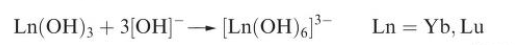
\includegraphics[scale=1]{gg1}}
\end{figure}
\begin{figure} [H]
	\centering {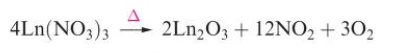
\includegraphics[scale=1]{gg2}}
\end{figure}
\begin{figure} [H]
	\centering {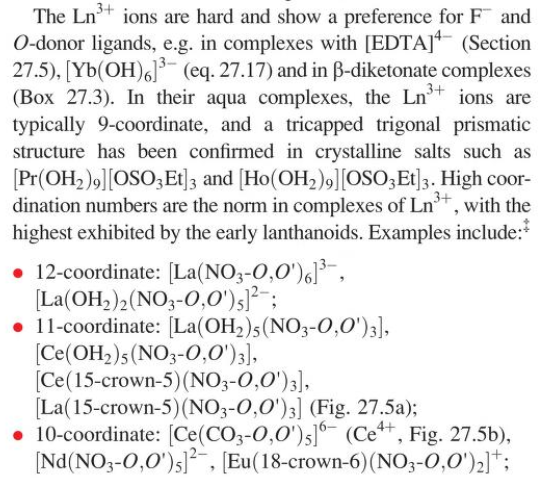
\includegraphics[scale=1]{gg3}}
\end{figure}
\begin{figure} [H]
	\centering {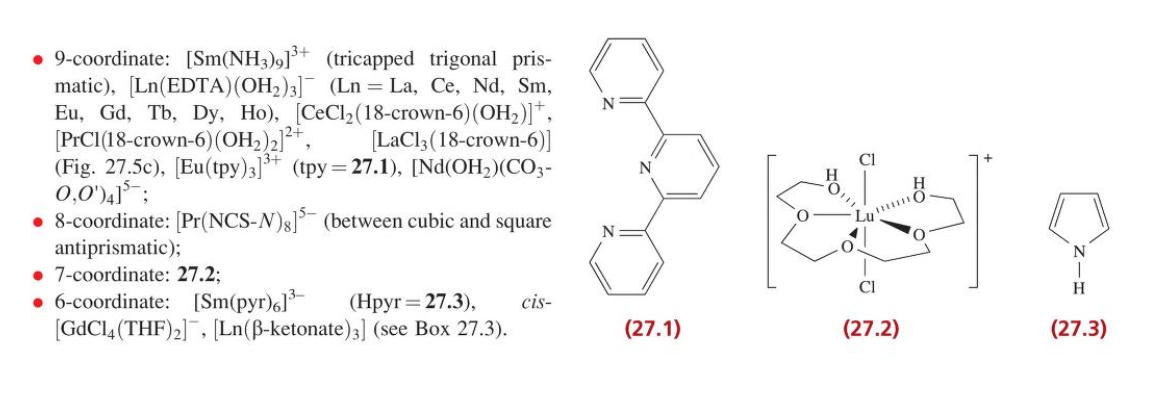
\includegraphics[scale=0]{gg4}}
\end{figure}
\begin{figure} [H]
	\centering {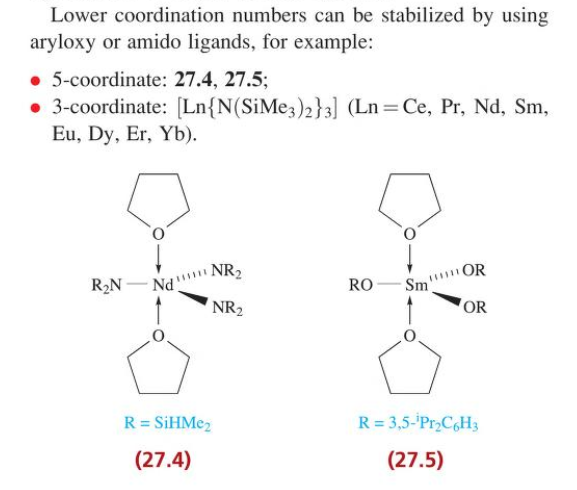
\includegraphics[scale=1]{gg5}}
\end{figure}
\begin{figure} [H]
	\centering {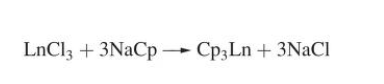
\includegraphics[scale=1]{gg6}}
\end{figure}
\begin{figure} [H]
	\centering {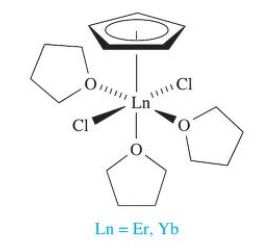
\includegraphics[scale=1]{gg7}}
\end{figure}
\begin{figure} [H]
	\centering {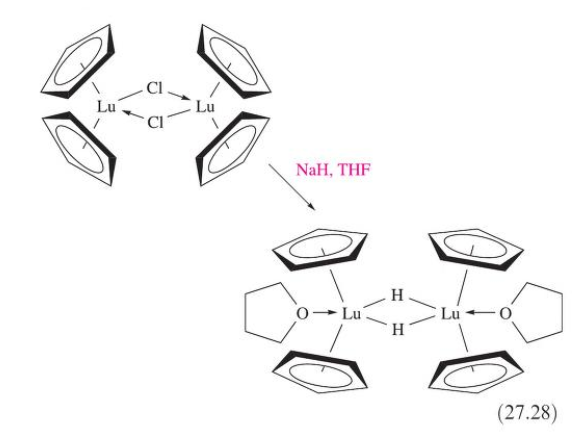
\includegraphics[scale=1]{gg8}}
\end{figure}


